%%%%%%% SECTION %%%%%%%
\section{Architecture de communication hybride}

%\subsection{Introduction}

Dans la section précédente, l'introduction du modèle orienté évènement s'intéresse 
principalement à ce qui se passe au sein d'un seul client. Or, la collaboration 
passe par la mise en relation des différents collaborateurs et l'échange des 
données nécessaires à la collaboration : données de connexion, mises à jour de la 
scène, sensibilisation \dots 

Afin de pouvoir proposer un \gls{SEC} adapté aux besoins de l'édition de scènes 
3D, plusieurs critères doivent êtres respectés: 
\begin{itemize}
	\item granularité fine pour l'édition massive;
	\item spécifique à la modélisation 3D;
	\item reposant sur des technologies web (réseau, interface, interaction 3D).
\end{itemize}

Les \gls{SEC} ont connu un fort développement avec l'intérêt croissant 
pour le \gls{P2P} dans les années 2000. 
La base théorique des \glspl{SEC} s'appuie sur les propriétés de 
convergence, préservation de la 
causalité et préservation de l'intention du modèle \acrshort{CCI} 
\cite{Sun1998} (cf Section \ref{sec:cci}). 
La plupart des travaux liés aux \gls{SEC} \gls{P2P} s'intéressent à 
l'édition collaborative massive de documents textuels dont les propriétés 
de commutativité sont plus faciles à gérer (insertion/suppression) en 
comparaison à celles concernant la 3D (multiplication de matrices de 
rotation). La génération de conflit en 3D peut vite devenir écrasante. Il est 
donc nécessaire de mettre en place des mécanismes de détection de 
conflit et de maintient de cohérence au cours des sessions de 
collaboration. 
Cela passe par la mise en place une architecture de communication 
hybride pour la collaboration. 
Le terme \og hybride\fg{} invoque un compromis entre la 
centralisation de l'information nécessaire à la prise de décision globale et 
la décentralisation des échanges utile à l'amélioration du partage de 
contenu 3D à l'échelle locale. 
En agissant sur ces deux échelles la granularité de la collaboration est plus fine. 
Par exemple, le passage à l'échelle est facilité par la présence de 
ressources locales et la coordination des utilisateurs se fait à une échelle 
globale ce qui permet également l'accès à une source de vérité 
centralisée (base de données) et commune.

Cette section décrit le modèle d'architecture mis en 
place pour gérer la transmission de contenu entre les différents clients 
participant à l'édition collaborative d'un espace de travail 3D. 
Ces travaux s'inscrivent dans un contexte où les besoins d'interopérabilité 
et de standardisation sont élevés pour permettre à des utilisateurs de 
prendre le système rapidement en main sans installer autre chose qu'un 
navigateur. 

\subsubsection{Constat}

\gls{WebRTC} est une technologie qui fournit aux navigateurs 
\textit{destkop} et mobiles la possibilité de communiquer en temps-réel 
(\textit{Real-Time Communications}) via une collection de standards, 
protocoles et \glspl{API} JavaScript. 
Le standard \gls{WebRTC} est développé au sein du \gls{W3C} et de 
l'\gls{IETF} depuis 2011 dans sa version 1.0 (Working Draft). 
L'un des atouts de cette technologie est de permettre de façon simple et 
sans module d'extension la capture d'un flux audio et / ou vidéo (ex : 
applications de VoIP), ainsi que l'échange de données arbitraires entre 
navigateurs sans nécessiter d'intermédiaires (ex : partage de fichier en 
P2P).
Techniquement, \gls{WebRTC} supporte un canal temps-réel 
bidirectionnel pour l'échange de données. Contrairement à 
\gls{WebSocket}, qui est basé sur \gls{TCP}, \gls{WebRTC} se base sur 
\acrshort{UDP} en intégrant une pile de plusieurs protocoles (Figure 
\ref{fig:protocolstack}) qui lui offre des fonctionnalités similaires (fiabilité, 
ordonnancement, sécurité). 

La jeunesse du protocole (2011) fait que peu de travaux académiques 
l'utilisent pour créer des \gls{EVC3D} \cite{Desprat2015a,Steiakaki2016}. 
Côté commercial, un grand nombre d'applications et de services 
basés sur ce protocole ont fait leur apparition (par ordre d'importance) : 
des systèmes d'échanges audio/vidéo (VoIP)\footnote{WebRTCWorld en 
	liste un peu plus de 140 
	\url{http://www.webrtcworld.com/webrtc-list.aspx}. Consulté le 
	07/07/2017.}, des systèmes de partage de fichiers\footnote{WebTorrent 
	\url{https://github.com/feross/webtorrent}. Consulté le 04/09/2017.} et 
autres applications (capture d'écran, réalité augmentée, jeux)
\footnote{Curation de ressources et modules WebRTC 
	recensant plus de 100 projets 
	\url{https://github.com/openrtc-io/awesome-webrtc}. Consulté le 
	07/07/2017.}. 

La simplicité de la mise en place (très semblable à WebSocket) et la 
richesse apportée par le \gls{P2P} n'y sont pas étrangers.
Les réseaux \gls{P2P} ne sont souvent pas bien connus des 
développeurs web qui sont habitués aux architectures client-serveur, ce 
qui peut représenter une barrière d'entrée pour de nouvelles applications 
réseau. 
Dans les systèmes \gls{P2P}, il n'y a pas de fermes de serveurs comme 
il peut en exister dans les applications client-serveur. 
Les machines clientes et les systèmes d'extrémité (\textit{end system}) 
sont considérée comme \og les ressources\fg{} dans un réseau 
\gls{P2P}. 
En principe, ces ressources sont difficilement administrables à l'échelle 
dans un réseau non structuré ; la qualité de service peut en pâtir.
Cependant, lors d'un déploiement \gls{P2P} réel, des serveurs sont en 
général utilisés pour télécharger l'application cliente qui contient la couche 
intergicielle \gls{P2P} et fournit à l'utilisateur le service de connexion 
nécessaire à l'accès au service. 
Ces serveurs sont moins coûteux que peut l'être une ferme de serveurs. 
De plus, pour beaucoup de services décentralisés, il n'existe 
pas de solution pérenne pour tester ces applications à l'échelle ; chaque 
service doit créer son propre système de test. 

Ce contexte technologique est un motivation supplémentaire dans les travaux de 
cette thèse.

%TODO parler chargeet distribution
\begin{figure}[th]
	\centering
	\includegraphics[width=0.8\columnwidth]{protocol_stack2.eps}
	\caption{Pile des protocoles IP: TCP vs UDP}
	\label{fig:protocolstack}
\end{figure}

\subsubsection{Contribution}
Une architecture de communication hybride en trois parties serveur, persistance, 
pairs est utilisée dans 3DEvent \cite{Desprat2016}. Cela permet de concilier à la 
fois les avantages d'une architecture client-serveur et ceux du \gls{P2P} en évitant 
certains désavantages occasionnés dans ceux-ci (engorgement du serveur, pair 
seul sur le réseau\dots). Dans le contexte des \gls{EVC} \gls{3D}, le but 
est d'obtenir une architecture de communication : 

\begin{itemize}
	\item entièrement basée web, 
	\item robuste à l'évolution du nombre de collaborateurs, 
	\item efficace en terme de d'accès et distribution de la donnée, 
	\item et qui s'adapte à l'échelle selon les besoins de la collaboration.
\end{itemize}

Dans cette section, les différents composants de l'architecture sont détaillés. 
Ensuite sont expliqués les mécanismes de mise en relation de 
ces composants pour que les différents participants d'une session 
collaborative puissent se communiquer de manière transparente, cohérente et 
résistante aux pannes.


\subsection{Présentation générale}
Un intergiciel (\textit{middleware}) se compose en général d'une API de 
recherche \ref{fig:middleware}.
Dans notre modèle cette brique est principalement en lien avec le 
gestionnaire d'instance qui se charge de la recherche. L'API de messagerie 
concerne plus directement le système d'envoie et de réception de message. Les 
différents message vont concerner la partie routage de l'information, le 
maintien à jour du répertoire de voisin et leur dynamicité, ainsi que la 
description des connexions à maintenir. Le bloc de gestion de session permet au 
pair de savoir avec qui il est connecté et contient également les méta informations 
liées à ces liens (temps de connexion). 
Chaque pair doit également posséder un endroit où stocker les information de 
contenu à traiter qui correspond à stockage de contenu. Cette dernière peut 
prendre plusieurs formes : in-memory, stockage local, disque dur\dots selon le 
type de stockage adapté et disponible.
Un pair est également au courant de son rôle. Le rôle d'un pair permet de 
distinguer s'il est un super pair, un pair normal, un pair actif, ou un pair passif\dots 
Le rôle induit les capacités et la configuration de chaque pair, i.e. un pair passif 
est configuré uniquement pour relayer les données tandis qu'un pair actif sera 
configurer pour traiter et relayer les données tandis qu'un pair passif ne fait que 
stocker et relayer les données.
\begin{figure}[ht]
	\centering
	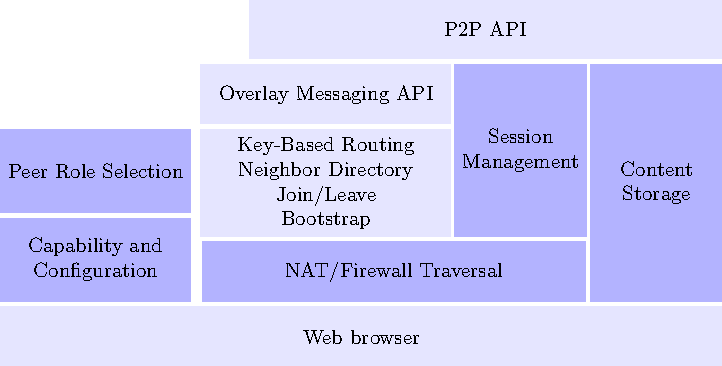
\includegraphics[width=0.7\textwidth]{tikz/middleware/middleware}
	\caption{Composants de chaque pair dans 3DEvent (point de vue réseau)}
	\label{fig:middleware}
\end{figure}

Le serveur assure d'une part la centralisation du stockage à long-terme et d'autre 
part la mise en relation des différents clients.

La couche \gls{P2P} fournit une dissémination rapide de l'information et 
décentralise la réplication des données à court terme. Cela évite donc au serveur 
d'être le point central des échanges en déchargeant les canaux passant par le 
serveur.

\paragraph{Connexion des pairs en début de session}

La Figure \ref{fig:connexionpairs} représente la séquence d'actions nécessaire à 
une instance 3DEvent ($idA$) pour rejoindre le réseau contenant déjà d'autres 
instances 3DEvent. L'action \textit{join} est exécutée lorsqu'un utilisateur envoie 
ses informations de connexion sur portail de connexion (à partir d'une instance 
web) ou lorsqu'une instance serveur est lancée. Cette action ajoute le nouveau 
pair à la liste des pairs présents sur le réseau, gérée par le gestionnaire 
d'instance, et retourne la liste des pairs avec lesquels le pair doit se connecter. 
Pour chaque pair $idB$ de la liste retournée $ids$, $idA$ utilisé le mécanisme de 
signalisation (offre/demande). Le mécanisme est déclenché par l'instanciation d'un 
\textit{network bridge}\info{definir} dans l'\textit{event store} \info{definir} de $idA$ 
puis celui de $idB$. Afin de resynchroniser les deux pairs (après cette série 
d'échanges asynchrones), $idA$ et $idB$ s'échanges des métadonnées sur la 
situation respective de leurs \textit{ESM} \info{definir} afin de se synchroniser 
\info{(see refernece sync mechanism}.

\begin{figure}[t]
	\noindent
	\centering
	\includegraphics[width=\textwidth]{connection.eps}
	\caption{Protocole de connexion au réseau d'instance 3DEvent}
	\label{fig:connexionpairs}
\end{figure}

\subsection{Event Store}

L'Event Store est un composant clé dans le traitement des évènements. Il prend 
en entrée des évènements générés ou reçus extérieurement et produit en sortie 
des évènements cohérents qui peuvent être par la suite publiés. Les évènements 
sont considérés comme cohérents lorsqu'il n'y a pas d'erreur de cohérence, i.e. 
lorsque les numéros de versions sont bien ordonnés. Chaque Event Store contient 
deux éléments: l'Event Stream Manager (ESM) et des Network Bridges (NB). Un
ESM est une structure de données représentée par une collection de flux 
d'évènements. Un flux d'évènement est représenté par un tableau d'évènements 
indexés en séquence permettant de stocker les évènements d'un aggrégat dans 
l'ordre temporel. Si un flux ne rencontre pas de problème de cohérence alors le 
dernier index correspond au numéro de version de l'agrégat. Lorsque l'Event Store 
reçoit un évènement de l'instance courante\info{utilisation du terme 
	instance?}, l'ESM récupère (ou crée) le flux d'évènements associé à l'agrégat 
référencé par l'évènement. Alors, la cohérence de la version est vérifiée en 
comparant la version attendue (exposée dans les métadonnées de l'évènement) 
et la version actuelle de l'agrégat. Si les deux numéros de versions sont égaux, 
l'évènement est ajouté à la fin tableau du flux pour être stocké, sinon une 
exception est levée. La gestion des exceptions est expliquée dans \info{détails 
	exception}. Une fois le stockage effectué dans l'ESM, l'évènement est publié.



\subsection{Persistance à long terme}\label{sec:persistance-a-long-terme}
Dans un contexte de collaboration sur le long terme pour des entreprises où le 
besoin d'information accessible sur le long terme est nécessaire. La persistance 
long-terme stocke le journal d'évènement qui est la 
source de vérité de l'application. Elle peut également stocker des projections 
prédéfinies, calculées à la volée ou encore des \textit{snapshots} de l'application.

\subsection{Synchronisation 
client-serveur}\label{sec:synchronisation-client-serveur}
Lors de la connexion d'un nouveau client a lieu la synchronisation des deux 
systèmes de persistance pour obtenir les mises à jour : 
\improve{l'échange des mises à jour entre le client (persistance à court terme) et la 
base de données (à long terme) afin de synchroniser les deux éléments avec. La 
base de données peut également servir en cas de conflit important ; elle sert de 
référent.}
\improve{synchro- nizing with a NoSQL-based database whenever possible 
(thereby supporting intermittent connections of mobile devices; this approach is 
known as “offline first”) \cite{Gadea2016}}
\begin{enumerate}
	\item depuis le client, où l'on distingue trois cas :
	\begin{enumerate}
		\item travail "\textit{offline}" (hors ligne) : l'utilisateur a travaillé hors ligne et 
		doit maintenant publier "en ligne" son travail. Les mises à jour publiées sur la 
		base de données ; le serveur vérifie si aucun conflit ne survient puis 
		fusionne (\textit{merge}) les nouvelles entrées avec l'existant; 
		
		\item travail "\textit{serverless}" (en collaboration avec d'autres pairs sans le 
		serveur) : dans le cas où le serveur est absent, les clients peuvent continuer 
		de créer en collaborant. Ces données n'étant stockées que sur le client, il est 
		de les transmettre à la base de données dès qu'une connexion est possible. 
		Cela peut être fait en une fois ou de manière partagée\improve{ça veut dire 
			quoi?};
		
		\item travail "\textit{online}" (en collaboration avec d'autres pairs avec le 
		serveur) : le client envoie régulièrement \improve{combien de temps} ses 
		nouvelles modifications pour qu'elles soient intégrées à la base de données.
	\end{enumerate}
	\item depuis la base de données :
	Le client reçoit toutes les nouvelles mises à jour de la scène depuis la dernière 
	fois qu'il s'est connecté. Cela peut également inclure des mises à jour qui sont 
	en conflit avec ce qu'il y a dans son propre espace de stockage qu'il lui faut 
	donc modifier.
	Dans le cas où un utilisateur est seul connecté, la base de données est la 
	seule source disponible pour la mise à jour du client. 
\end{enumerate}
\subsection{Gestion de la cohérence}


\subsubsection{Respect de la causalité}
\subsubsection{Convergence des répliques}
\subsubsection{Préservation de l'intention}
\subsection{Bilan}